% mnras_template.tex 
%
% LaTeX template for creating an MNRAS paper
%
% v3.0 released 14 May 2015
% (version numbers match those of mnras.cls)
%
% Copyright (C) Royal Astronomical Society 2015
% Authors:
% Keith T. Smith (Royal Astronomical Society)

% Change log
%
% v3.0 May 2015
%    Renamed to match the new package name
%    Version number matches mnras.cls
%    A few minor tweaks to wording
% v1.0 September 2013
%    Beta testing only - never publicly released
%    First version: a simple (ish) template for creating an MNRAS paper

%%%%%%%%%%%%%%%%%%%%%%%%%%%%%%%%%%%%%%%%%%%%%%%%%%
% Basic setup. Most papers should leave these options alone.
\documentclass[fleqn,
%referee, % this line changes to double-spaced 1 column
usenatbib]{mnras}


% MNRAS is set in Times font. If you don't have this installed (most LaTeX
% installations will be fine) or prefer the old Computer Modern fonts, comment
% out the following line
\usepackage{newtxtext,newtxmath}
\usepackage{anyfontsize}
% Depending on your LaTeX fonts installation, you might get better results with one of these:
%\usepackage{mathptmx}
%\usepackage{txfonts}

% Use vector fonts, so it zooms properly in on-screen viewing software
% Don't change these lines unless you know what you are doing
\usepackage[T1]{fontenc}

% Allow "Thomas van Noord" and "Simon de Laguarde" and alike to be sorted by "N" and "L" etc. in the bibliography.
% Write the name in the bibliography as "\VAN{Noord}{Van}{van} Noord, Thomas"


%%%%% AUTHORS - PLACE YOUR OWN PACKAGES HERE %%%%%

% Only include extra packages if you really need them. Common packages are:
\usepackage{graphicx}	% Including figure files
\usepackage{amsmath}	% Advanced maths commands
% \usepackage{amssymb}	% Extra maths symbols
\usepackage{hyperref}
\usepackage[normalem]{ulem}
\usepackage[dvipsnames]{xcolor}
% \usepackage{enumitem}

\usepackage{tikz}


\graphicspath{{figures/}} 
% \linespread{1.8}




%%%%%%%%%%%%%%%%%%%%%%%%%%%%%%%%%%%%%%%%%%%%%%%%%%

%%%%% AUTHORS - PLACE YOUR OWN COMMANDS HERE %%%%%

% Please keep new commands to a minimum, and use \newcommand not \def to avoid
% overwriting existing commands. Example:
%\newcommand{\pcm}{\,cm$^{-2}$}	% per cm-squared


% citations
\defcitealias{james+21}{J21}
\newcommand{\JJ}{\citetalias{james+21}}
\newcommand{\VICE}{\textsc{vice}}


\newcommand{\fruity}{\texttt{\hyperlink{fruity}{Fruity}}}
\newcommand{\nugrid}{\texttt{\hyperlink{nugrid}{NuGrid}}}
\newcommand{\monash}{\texttt{\hyperlink{monash}{Monash}}}
\newcommand{\aton}{\texttt{\hyperlink{aton}{ATON}}}
\newcommand{\cfactor}{1.44}
\newcommand{\nsubgiants}{14,069}



% Acronyms
\newcommand{\agb}{AGB}
\newcommand{\apogee}{APOGEE}
\newcommand{\aspcap}{\textsc{aspcap}}
\newcommand{\cc}{CCSN}
\newcommand{\gce}{GCE}
\newcommand{\ia}{SN Ia}

% internal abbreviations
\newcommand{\caah}{[C/Mg]-[Mg/H]}
\newcommand{\caafe}{[C/Mg]-[Mg/Fe]}


% other
\newcommand{\ycmg}{\ensuremath{2.7 + 32\left(Z-\Zo\right)}}
\newcommand{\fmeas}{20\%}

\makeatletter
\newcommand{\C}[1][\@nil]{
    \def\tmp{#1}%
    \ifx\tmp\@nnil%
        \ensuremath{\rm C}%
    \else%
        \ifmmode ^{#1}{\rm C}%
        \else $^{#1}$C%
        \fi%
\fi }
\makeatother

\newcommand{\Yct}{{y_{\rm C}}}
\newcommand{\Ycc}{{y_{\rm C}^{\rm CC}}}
\newcommand{\Yoc}{{y_{\rm Mg}^{\rm CC}}}
\newcommand{\Ycagb}{{y_{\rm C}^{\rm AGB}}}
\newcommand{\aagb}{\alpha_{\rm C}^{\rm AGB}}
\newcommand{\zagb}{\zeta_{\rm C}^{\rm AGB}}
\newcommand{\zcc}{\zeta_{\rm C}^{\rm CC}}
 \newcommand{\yb}{\ensuremath{\rotatebox[origin=B,y=0.5ex]{180}{y}}}
\newcommand{\y}{Y}
\newcommand{\fagb}{f_{\rm C}^{\rm AGB}}

\newcommand{\Mo}{ {\rm M}_{\sun}}
    
\newcommand{\Zo}{ Z_{\sun}}

\newcommand{\about}[1]{${\sim} #1$}

%%% citepos command
\makeatletter
\DeclareRobustCommand\citepos
  {\begingroup
   \let\NAT@nmfmt\NAT@posfmt% ...except with a different name format
   \NAT@swafalse\let\NAT@ctype\z@\NAT@partrue
   \@ifstar{\NAT@fulltrue\NAT@citetp}{\NAT@fullfalse\NAT@citetp}}

\let\NAT@orig@nmfmt\NAT@nmfmt
\def\NAT@posfmt#1{\NAT@orig@nmfmt{#1's}}

\makeatother


% Caption macros
\newcommand{\captionline}[2][very
thick]{\tikz[baseline={([yshift=-.5ex]current bounding box.base)}]{
\draw[#2,#1, line cap=round] (0,0) -- (0.3,0); }}




%%%%%%%%%%% JWJ' editing macros %%%%%%%%%%%
\newcommand{\strike}[1]{{\color{ForestGreen} \sout{#1}}}
\newcommand{\add}[1]{{\color{ForestGreen} #1}}
\newcommand{\note}[1]{{\color{ForestGreen} \textit{ \small (JWJ: #1)}}}
% \LetLtxMacro\origcitep\citep
% \LetLtxMacro\origcitet\citet
% \renewcommand{\citep}[2][]{%
%     \mbox{\origcitep[#1][]{#2}}
% }
% \renewcommand{\citet}[2][]{%
%     \mbox{\origcitet[#1][]{#2}}
% }

\newcommand{\dbstrike}[1]{{\color{Thistle} \sout{#1}}}
\newcommand{\dbadd}[1]{{\color{Thistle} #1}}
\newcommand{\dbnote}[1]{ {\color{Thistle} \textit{\small (DB: #1)}} }


% \LetLtxMacro\origcite\cite

% This is my command. I want to strike out, 
% \newcommand{\strikeit}[1]{%
%   \ifcorrectingmode
%   \mbox{\sout{#1}}%
% %  \makebox[\textwidth][s]{\sout{#1}}%
%   \fi
% }

% \renewcommand{\cite}[2][]{%
%   \ifcorrectingmode
%   \mbox{\origcite[#1]{#2}}%
%   \else
%   \origcite[#1]{#2}%
%   \fi
% }




%%%%%%%%%%%%%%%%%%%%%%%%%%%%%%%%%%%%%%%%%%%%%%%%%%

%%%%%%%%%%%%%%%%%%% TITLE PAGE %%%%%%%%%%%%%%%%%%%

% Title of the paper, and the short title which is used in the headers.
% Keep the title short and informative.
\title[The Origin and Galactic Evolution of Carbon]{The Galactic Chemical Evolution of Carbon: Implications for Stellar Nucleosynthesis }

% The list of authors, and the short list which is used in the headers.
% If you need two or more lines of authors, add an extra line using \newauthor
\author[D. A. Boyea et. al.]{%
Daniel A. Boyea,$^{1, 2, 3}$\thanks{%
Contact e-mail:~\href{mailto:boyea.2@osu.edu}{boyea.2@osu.edu}}
James W. Johnson,$^{1, 2, 4}$
Third Author$^{2,3}$
and Others$^{1,3}$
\\
% List of institutions
$^{1}$Department of Astronomy, The Ohio State University, 140 W. 18th Ave., Columbus, OH, 43210, USA
\\
$^{2}$Center for Cosmology \& Astroparticle Physics (CCAPP), The Ohio State University, 191 W. Woodruff Ave., Columbus, OH, 43210, USA
\\
$^{3}$Department of Physics \& Astronomy, University of Victoria, Victoria, BC V8P 5C2, Canada
\\
$^{4}$The Observatories of the Carnegie Institution for Science, 813 Santa Barbara St., Pasadena, CA, 91101, USA
}

% These dates will be filled out by the publisher
\date{Accepted XXX. Received YYY; in original form ZZZ}

% Enter the current year, for the copyright statements etc.
\pubyear{2024}

% Don't change these lines
\begin{document}
\label{firstpage}
\pagerange{\pageref{firstpage}--\pageref{lastpage}}
\maketitle



% Abstract of the paper
\begin{abstract}
% context
The origin of C, despite its importance, remains poorly understood. 
% 
We aim to constrain the stellar yields of C through multi-zone Galactic chemical evolution models by comparing predictions with \apogee\ subgiants abundances.
% 
We find that \caafe\ trends, when restricted in metallicity, are an empirical estimate of the delayed C sources, enabling us to estimate that \agb\ stars and \cc\ produce about 20\% and 80\% of C, respectively.  
The \caah\ trend instead represents the equilibrium abundances of C and Mg. 
We use the \caah\ trend to estimate the CCSNe C/Mg yield, determining that  $\Ycc/\Yoc = EQUATION$ when including \agb\ C. 
% misc
Our models are relatively independent of uniform scaling of yields and outflows, and alternate star formation histories. 
However, the stars which contribute to \agb\ C production and the \ia\ delay time distribution of Fe contribute uncertainties to our conclusions. 
% gas phase
While reliable gas-phase and low-metallicity measurements of C are challenging, we find that our model and a single-zone model with our recommended yields replicate the broad trends of \caah{} across different environments and metallicities. 

\end{abstract}

\begin{keywords}
galaxies: abundances -- galaxies: evolution -- galaxies: star formation -- galaxies: stellar content -- methods: numerical
\end{keywords}



%%%%%%%%%%%%%%%%%%%%%%%%%%%%%%%%%%%%%%%%%%%%%%%%%%

%%%%%%%%%%%%%%%%% BODY OF PAPER %%%%%%%%%%%%%%%%%%

\section{Introduction}


\begin{figure*}
    \centering
    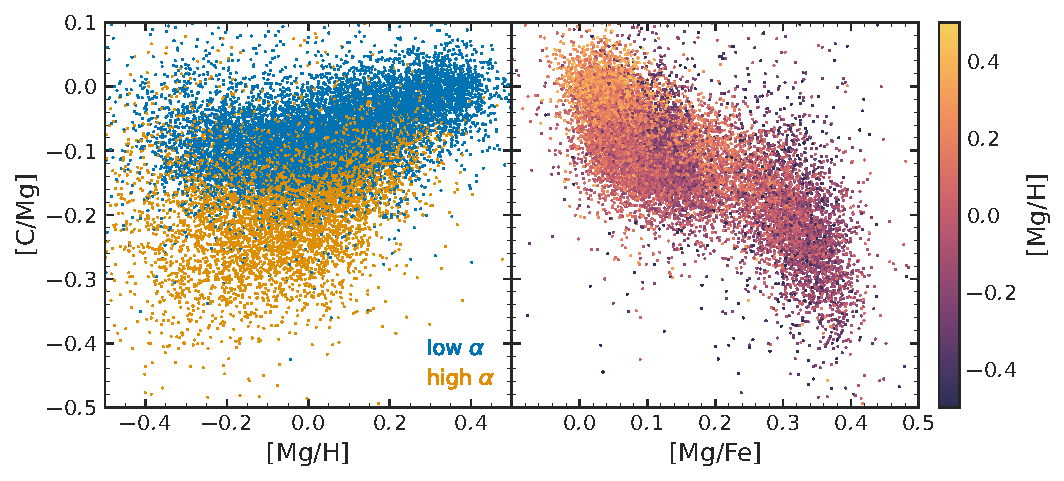
\includegraphics{subgiants.pdf}
    \caption{The [C/Mg] ratio against [Mg/H] (left) and [Mg/Fe] (right) for the \citet{jack}~sample of \apogee{} subgiants. On the left, we plot high and low-$\alpha$ stars in blue and orange, using the separation defined in Equation \ref{eq:high_alpha} \dbstrike{(the high and low-$\alpha$ stars are named for their high or low $\alpha$-element (Mg) to Fe ratios)}. On the right, we colour-code stars according to their [Mg/H] abundance.} \label{fig:subgiants}
\end{figure*}



Despite being the most abundant metal in the Universe~\citep[e.g.][]{magg+22}, the nucleosynthetic origin of C is inadequately understood. \dbnote{need synonyms for poorly understood}
Broadly, studies agree that both high mass and asymptotic giant branch (AGB) stars produce C, but their relative yields are disputed.
From a Galactic chemical evolution (GCE) perspective, some authors have argued that high-mass stars should dominate~\citep[e.g.][]{prantzos+94, HEK00, romano+20, franchini+20, gustafsson22}, and others have argued that AGB stars should contribute at least half of the C in the universe~\citep[e.g.][]{tinsley79, chiappini+03, mattsson10, KKU11, rybizki+17, KKL20}. 
\dbadd{We aim to empirically characterize the yields of C and the ratio of AGB and CCSNe production.}

% Formed in the cores of stars during He fusion, C is the first \dbadd{primary? element} after He. Additionally, C is one of the only light elements formed in low-mass stars \citep[e.g.,][]{KL14}. \dbnote{I don't like how many e.g.'s there are, and is this the right citation here?}
%\dbadd{
% Because the effects of first dredge up are mass-dependent, C and N abundances are frequently used as age indicators for RGB stars \citep{MG15, martig16, hasselquist19, vincenzo+21}. 
% }
% \dbnote{C abundnces for stellar structure (opacities) and star formation (line cooling)}



Predictions of C yields from stellar evolution and supernova (SN) models are riddled with uncertainties (see, e.g., the reviews/summaries by \citealt{romano+10, KL14}).
Stellar yields are shaped by many poorly understood processes, such as mass loss rates \citep{sukhbold+16, beasor+2020}, rotational mixing \citep{frischknecht+16, LC18}, reaction rates \dbadd{citations}, and convection \citep{chieffi2001, ventura+13}.
\dbnote{I checked these, is sukhbold the best reference on mass loss?}
\dbadd{In addition, stellar parameters such as convection and mass loss are calibrated to match observed stars and cannot be predicted from first principles.} \dbnote{need to check if this means SE models are calibrated to match yields or just stellar parameters.}
Small changes in the initial mass of only $\sim$$0.01 M_\odot$  were recently shown to have dramatic effects on the evolution and explosion outcomes of massive stars \citep{bruenn+2023, vartanyan_burrows2023}.
Furthermore, many stars are found in binary systems \dbadd{(e.g. \citealt{MKB2019}, others?)}, the effects of which are almost entirely unexplored in stellar nucleosynthesis models \citet{farmer+21}.
Therefore, accurate yield predictions from stellar theory requires both a much greater understanding of stellar physics and a much more densely sampled grid of models than is currently available.


In light of the challenges of stellar theory, recent work has instead sought to characterize chemical yields empirically.
\citet{HLA20} measured the abundance ratios in the ejecta of Cassiopeia A using spatial resolved X-ray spectra.
\citet{weinberg+19, weinberg+22} analyzed the abundance ratio trends of high- and low-alpha sequence stars in APOGEE~\citep{apogee17} to infer relative yields of prompt and delayed enrichment sources and the metallicity dependence thereof.
\citet{emily+19, emily+22, emily+24} applied the same methodology to GALAH~\citep{DeSilva2015, Martell2017}.
\citet{rodriguez+21, rodriguez+23} measured the mean Fe yield of core-collapse supernovae (CCSNe) using the radioactive tails of their lightcurves.
\dbnote{even papers as far back as at least https://ui.adsabs.harvard.edu/abs/1997NuPhA.621...27G/abstract do this. Include this series as well: https://ui.adsabs.harvard.edu/abs/2023MNRAS.525.1329L/abstract}


% \note{Reading through at least at this moment, I'd say this is a reasonable place for a new paragraph. I wouldn't worry about referencing Weller et al. (2024) since He chemical evolution is not super relevant here.}
 Folowing many previous works  (e.g. \citealt{DTS78, BF06, prantzos+18, berg+19}; see also the recent reviews by \citealt{romano22} and \citealt{RM21}.) this paper focuses on the evolution of C in GCE models.
Most notably for our purposes, \citet{james+23} recently showed that the enrichment history of the Galactic disk can be described as an equilibrium phenomenon.
In equilibrium GCE, trends in abundance ratios with metallicity arise as a consequence of trends in yield ratios (see discussion in their section {\color{red} X.Y}).
\citet{james+23} had previously shown that the correlation between gas-phase N and O abundances (see their Fig. 1) could be described as a consequence of the metallicity dependence of the relative N and O yields.
The equilibrium scenario suggests that this argument should extend to any element whose enrichment by stellar populations does not require long timescales ($\gtrsim$few Gyr).
We therefore extend \citepos{james+23} arguments to C, which is closely related to N.


We use a sample of subgiant stars from APOGEE \citep{apogee17} as our primary observational constraint.
\dbadd{APOGEE Subgiants provide a large, homogenous sample of well-measured C abundances unaffected by stellar evolution}.
Subgiants advantageously have photospheric abundances directly representing birth C abundances \citep{gilroy89, korn+07, lind+08, souto+18, souto19}.
In other evolutionary phases, the measured abundances are known to be affected by internal processes (see discussion in section 2 below), namely gravitational settling in main sequence stars {\color{red} (reference)} and dredge-up in red giants {\color{red} (reference)}, 
Our sample should greatly mitigate these difficulties with inferring birth abundances of C, which have been a significant source of uncertainty for previous investigations of its nucleosynthetic origin.

% \dbnote{not sure the observations below need to be  too detailed here? Maybe just state that C/O appears to have a universal shape across environments and direct to that section since our main focus is on APOGEE? and disk chemistry?  }
% \dbstrike{
% From observations of nearby stars and (extragalactic) gas, we know that [C/O] against [O/H] traces a banana shape (see Fig.~\ref{fig:gas_phase} and section~\ref{sec:gas}).
% At the very lowest metallicities ($[{\rm O/H}]\lesssim-2$),%
% %
% observations indicate that [C/Mg] declines with metallicity.
% From $-2 \lesssim {\rm [O/H]}\lesssim -1$, [C/Mg] is roughly constant with metallicity. 
% At higher metallicities ([O/H]~$\gtrsim -1$), [C/Mg] increases with metallicity.
% }
% \dbstrike{We will show in section~\ref{sec:results} below that these correlations in the bulk population abundances alone are quite constraining for the origin of C.}


In Section~\ref{sec:data_selection} we describe the selection for our subgiant observational sample.
Section~\ref{sec:nucleosynthesis} discusses theoretical estimates of \agb\ and \cc\ C yields. We parameterize our yield choices and derive a estimate of C/Mg yields observationally.
Section~\ref{sec:vice} reviews the multizone model and modifications thereof for this work.
Section~\ref{sec:results} presents our multizone model predictions and GCE parameters which are observationally permissable. 
Finally Section~\ref{sec:gas} compares our model to literature collected observations of halo stars and extragalactic HII regions. 




\footnotetext{In this paper, we use the standard notation for chemical abundances. $[A/B] = \log_{10}\left(A/B\right) - \log_{10}\left(A_{\sun}/B_{\sun}\right)$, i.e. $[A/B]$ is the logarithm of the mass ratio between A and B, scaled such that $[A/B]=0$ for the sun (see Table~\ref{tab:fiducial_mod} for solar scale.) }

% \footnotetext{\strike{By metallicity, we mean the (mass) fraction of any element which is not H or He, denoted by $Z$. For the sun, we take $Z_\odot=0.016$.} }


\section{The Subgiant Sample}\label{sec:data_selection}




% Subgiants are a useful empirical benchmark because their photospheric abundances should reflect their birth mixture. 
As an emperical benchmark, we use subgiant stars, whose photospheres accurately represent birth abundances. 
During main sequence evolution, metals can fall to below the convective envelope (i.e., ``gravitational settling").
When stars leave the main sequence and become subgiants, these metals are mixed with the convective envelope \citep[]{gratton+00, souto19}. 
 \textit{First dredge up} during the red giant phase brings CNO processed core material to the surface \citep{iben67, KL14}.

We use the sample of \apogee\ DR17 subgiants from \citet{jack}, selecting stars from allStar-dr17-synspec\_rev1 within the $\log g$-$T_\text{eff}$ polygon given by
 \begin{equation}
    \begin{cases} \label{eq:subgiant_selection}
        \log \text{g} \geq 3.5 \\
        \log \text{g} \leq 0.004\,T_{\rm eff} - 15.7 \\
        \log \text{g} \leq 0.0007\,T_{\rm eff} + 0.36 \\
        \log \text{g} \leq -0.0015\,T_{\rm eff} + 12.05 \\
        \log \text{g} \geq 0.0012\,T_{\rm eff} - 2.8. \\
    \end{cases}
\end{equation}
Also following \citet{jack}, we exclude stars with the flags:
        \verb|APOGEE_MIRCLUSTER_STAR|,
        \verb|APOGEE_EMISSION_STAR|,
        \verb|APOGEE_EMBEDDEDCLUSTER_STAR|,
        \verb|APOGEE2_YOUNG_CLUSTER|,
        \verb|APOGEE2_W345|,
        \verb|APOGEE2_EB|, and
        \verb|DUPLICATE|.
We additionally remove stars with no reported C, Mg, or Fe abundances (in the {\tt X\_FE} columns). These cuts yield a sample containing \nsubgiants\ subgiants.


Fig.~\ref{fig:subgiants} shows the subgiant sample plotted in \caah\ and \caafe{}.\footnotemark{} In this sample, [C/Mg] increases with metallicity, and [C/Mg] decreases with [Mg/Fe] at fixed [Mg/H]. 

\dbadd{
Not shown here, we investigate the median trends for different samples and surveys, including APOGEE Giants with mixing corrections \citep{vincenzo+21}, APOGEE dwarfs, Gaia-ESO dwarfs, GALAH subgiants, LAMOST MRS (CITE), and smaller spectroscopic samples of stars. The predominant difference between any survey with our sample is a systematic offset in [C/Mg] in both [Mg/Fe] and [Fe/H] of at most 0.2 dex. The exception is GALAH, who's C abundances are highly incomplete, based on a single line and thus C measurements are likely unreliable (see e.g. Emily). If the median trend of [C/Mg] is offset from what we assume, then we can simply scale our C yields by the appropriate factor (e.g. -0.15 dex => $10^{-0.15} \approx 0.7$, so $y_{\rm C} \rightarrow  0.7 y_{\rm C}$) without significantly changing our results.
}

\section{Nucleosynthesis}\label{sec:nucleosynthesis}


Table \ref{tab:fiducial_mod} contains our fiducial yields and abundance scale. We use solar abundances from \citet{magg+22} with a +0.04 gravitational settling correction  and assuming $X_\odot= 0.71, \mu_{H} = 1$ as in \citet{david_fe}. We thus assume $Z_\odot=0.016$ as apposed to $Z=0.014$ in \citet{asplund+09}.
% Z = (1-Y) / (1 + X/Z)


\begin{table}
	\centering
    \caption[]{Solar abundance scale and fiducial yields (in units of SSP~birth mass). See section \ref{sec:agb} for the definition of \fruity. The solar abundance scale is \citet{magg+22} + 0.04. }
	\label{tab:fiducial_mod}

	\begin{tabular}{l l l l l}
		\hline
        Element & $Z_{X,\,\sun}$ & $y_X^{\rm cc}$ & $\y_X^{\rm agb}$ & $y_X^{\rm ia}$  \\
		\hline
        C & 0.00339 & Eq.~\ref{eq:y_cc} & $\cfactor\times$\fruity &  0 \\
        O & 0.00733 & 7.12e-3 & 0 & 0 \\
        Mg & 0.000671 & 6.52-4 & 0 & 0 \\
        Fe & 0.00137 & 4.72e-4 & 0 & 6.69e-4 \\
        N &0.00104 & 4.001e-4 & 0.0009$M\left(\frac{Z}{Z_\odot}\right)$ & 0\\
        % C & 0.00339 & Eq.~\ref{eq:zeta} & $\cfactor\times$\fruity &  0 \\
        % O & 0.00733 & 0.015 & 0 & 0 \\
        % Mg & 0.000671 & 0.00185 & 0 & 0 \\
        % Fe & 0.00137 & 0.0012 & 0 & 0.00214 \\
        % N &0.00104 & 0.00072 & 0.0009$M\left(\frac{Z}{Z_\odot}\right)$ & 0\\
		\hline
	\end{tabular}
\end{table}


We define a stellar yield as the fraction of a star's initial mass $M$ which is converted into freshly synthesized C. If $\Delta Z_{\rm C}$ represents the change in the mass fraction of C abundance, then the stellar yield is
\begin{equation}
    \y_{\rm C}^{\rm AGB} =  \Delta Z_{\rm C} \frac{M_{\rm ejected}}{M} = 
    \frac{W_{\rm C}(M) - Z_{\rm C}\, M_{\rm ejected}}{M}
\end{equation}
where $\Delta Z_{\rm C}$ represents the change in mean metallicity of the initial composition the star was born from, $M_{\rm ejected} = M - M_{\rm rem}$ is the total ejected wind mass through the stars lifetime, $W_{\rm C}$ is the total mass of C ejected through winds, and $Z_{\rm C}$ is the initial C mass fraction of the star. 
For CCSNe, 
\begin{equation} \label{eq:imf-cc-yield}
   Y_{\rm C}^{\rm CC}(Z) = 
    \frac{E(M)\,M_{\rm C}(M) + W_{\rm C}(M) - Z_{\rm C}\,M}{M}
\end{equation}
\dbnote{Is the - Z M term right or should M be Mzams - Mrem ?}
where $E(M)$ is the explodability function, $M_{\rm C}(M)$ is the mass ejected in a successful supernovae, and $W_{\rm C}$ and $Z_{\rm C}$ are as above.
We assume 8\,$\Mo$ is the minimum mass of \cc\ progeneters (see \VICE\ documentation and \citealt{emily+21}). 
Note that a yield may be negative if a star expels gas with lower $Z_{\rm C}$ than the star was born with. 



An IMF-averaged yield adds together the yields of stars of each mass, weighted by the fraction of stars of each mass (the IMF). 
The IMF-averaged yield $y_X^{\rm proc}$ for element $X$ under the enrichment process ${\rm proc}$ is given by
\begin{equation} \label{eq:imf-agb-yield}
    y_{X}^{\rm proc}(Z,\tau) = 
    \frac{
    \int_{M_{\rm to}(\tau)}^{M_{\rm max}} 
    \y_{\rm X}^{\rm proc}(M, Z) M\ 
    \frac{dN}{dM}\ dM
}
{
    \int_{M_{\rm min}}^{M_{\rm max}}\ M\ \frac{dN}{dM}\ dM
}
\end{equation}
where ${dN}/{dM}$ is the IMF and $M_{\rm to}(\tau)$ is the mass of stars with lifetime $\tau$, and $M_{\rm min}=0.08$ and $M_{\rm max} = 100$ are the assumed maximum and minimum values of the IMF.
$y$ thus represents the amount of freshly synthesized material returned to the ISM per unit of star formation. 
Note that in detail, the core collapse enrichment occurs on such short timescales that $M_{\rm to} = M_{\rm min, cc} = 8\,\Mo$


\subsection{Asymptotic Giant Branch Stars}\label{sec:agb}


\begin{figure*}
    \centering
 	    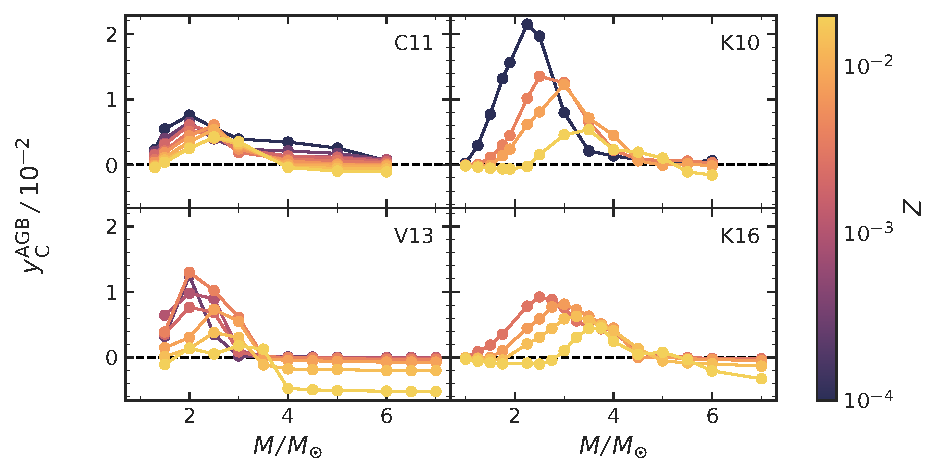
\includegraphics[scale=1]{agb_yields.pdf}
        \caption[]{\dbnote{replace y label with stellar C yield}. The net fractional \agb\ C yield  plotted as a function of initial stellar mass $M$ and colour-coded according to metallicity. The black dashed line shows $\y=0$ for reference. Each panel represents yields from one of four \agb\ models: \fruity{}, \aton{}, \monash{}, \nugrid{} (see sections \ref{sec:agb}) }

        \label{fig:y_agb}
\end{figure*}

\begin{figure*}
    \centering
    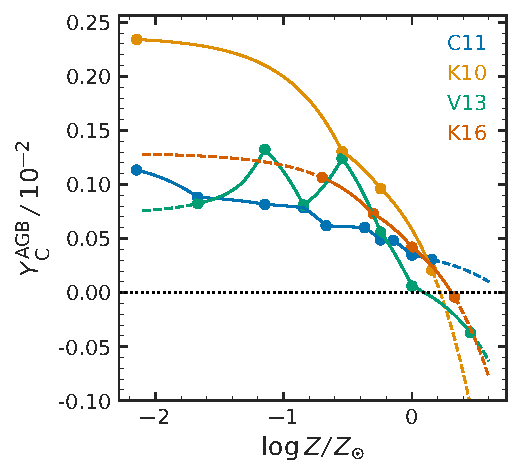
\includegraphics{y_agb_vs_z.pdf}
    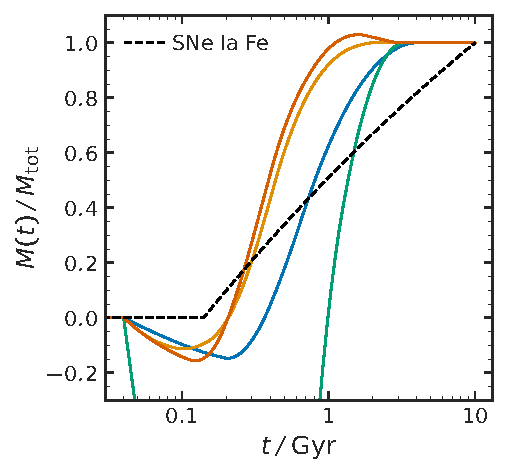
\includegraphics{y_agb_vs_t.pdf}

    \caption[]{\textbf{Left} \dbnote{ylabel: integrated carbon AGB yield} The (IMF-weighted) \agb\ C yield $\Ycagb$ as a function of metallicity for each of the \agb\ yield models. ($\Ycagb$ is the net mass of C produced by \agb\ stars per unit mass of star formation, after 10\,Gyr and assuming a \citealt{kroupa01} IMF.)
    \textbf{Right} cumulative C return as a function of age for a solar metallicity single stellar population. The dashed black line shows the delay time distribution of type Ia supernovae ($\propto t^{-1.1}$) for comparison. The minimum of \aton{} is $y(t)/y(t_{\rm end})=-46$. \dbnote{I think this changed with the new integration scheme...}
}

    \label{fig:agb-ssp}

\end{figure*}


An Asymptotic Giant Branch (AGB) star is a low mass star during its last nuclear (He shell) burning phase which enriches the interstellar medium (ISM) through mass loss during thermal pulses.(see e.g. \citealt{PR2023} \dbnote{or more introductory textbook like Ryden intro to astro?}) . 
In this work, we explore four different stellar AGB yield tables from the literature which provide well-sampled grids in mass and metallicity. We refer to the tables as 
\begin{description}
    \item \hypertarget{fruity}{\texttt{FRUITY}}: \citet{cristallo+11, cristallo+15}
    \item \hypertarget{aton}{\texttt{ATON}}: \citet{ventura+13,ventura+14,ventura+18, ventura+20}
    \item \hypertarget{monash}{\texttt{Monash}}: \citet{KL16, karakas+18}
    \item \hypertarget{nugrid}{\texttt{NuGrid}}: \citet{pignatari+16, ritter+18, battino+19, battino+21}
\end{description}
Table~\ref{tab:agb} notes the masses and metallicities for each grid of yields.
We use the same tables as \citet{james+23}, except that we have swapped \citet{karakas10} for \citet{pignatari+16}.


Fig.~\ref{fig:y_agb} compares the stellar \agb\ C yields for these four models.
Most models agree on general yield trends in mass and metallicity.
C production peak between masses of $\sim$ 2--4 $\Mo$ and declines as stars become more or less massive. As metallicity increases, the net yield decreases and the mass of peak C production increases slightly.

In order to integrate yields across the metallicity and mass range of interest, we interpolate yield tables linearly in both $Z$ and mass. Below the last sampled mass, $Y_{\rm C}^{\rm AGB}$ is linearly interpolated to 0 at $0.5\Mo$. The choice of yields for stars of masses $\Mo \lesssim 1.5$ produces about a 20\% uncertainty in the late DTD (past 3\,Gyr) of \agb\ C production from these models. More complete grids in mass and metallicity would be needed to more accurately compare GCE predictions between AGB evolution models. Furthermore, note the non-monotonic IMF-averaged yields in \nugrid\ and \aton\ particularly at low metallicities.

The left panel of Fig.~\ref{fig:agb-ssp} shows IMF-averaged C yields for each \agb\ model as a function of metallicity.
The \agb\ models mostly differ in their yield normalization and metallicity dependence.  
The normalizations span a factor of \about{2}.
For example, at $Z = 0.1\Zo$, each models predicts $Y_{\rm C}^{\rm AGB}$ to be between 0.0008 and
0.0016.
To characterize the metallicity dependence of each table, we fit the yield to a linear model in $\log Z$
\begin{equation}\label{eq:agb_z_approx}
    y_{\rm C}^{\rm AGB}(Z) = y_0 + \zagb \log(Z / \Zo).
\end{equation}
Table \ref{tab:agb} contains the fit parameters $y_0$ and $\zagb$ for each AGB table\footnote{we perform a MCMC fit using standard RMS error to estimate best parameters and uncertanties.}
The metallicity dependence of the yields span a factor of \about{3}.
Variations in \agb\ model yields are due to different choices of reaction rates, convection treatments, and mass-loss rates \citet{ventura+15} \dbnote{better ref here, is there a good review on AGB physics uncertanties?}.



The right panel of Fig.~\ref{fig:agb-ssp} shows the total production of C by \agb\ stars by a SSP as a function of age at solar metallicity. 
As the mass range $2\,\Mo\lesssim M \lesssim 4\,\Mo$ is most important for C production, half the yield is produced before \about{1}\,Gyr, similar to Fe production by \ia. 
\monash{} weight C production more heavily towards high-mass \agb\ stars, resulting in shorter delay times, whereas the \fruity\ and \aton\ models predict a slightly longer timescale of \about{1}\,Gyr. In any case, little to no C is produced more than 2\,Gyr after a star formation event. Fe production, in contrast, continues steadily for 10\,Gyr. 

In \agb\ stars, two competing processes determine the outcome of C production: {third dredge up} (TDU) and {hot bottom burning} (HBB).  
TDU accompanies thermal pulses in \agb\ stars, where material from the CO core is mixed with the envelope, increasing surface C abundances \citep{KL14}. The C yields of the star are increased as this C-enhanced envelope is released to the ISM. 
HBB\ is the activation of the CNO cycle at the bottom of the convective envelope. 
TDU increases C yields and HBB converts C into N. When both processes activate, highly efficient N production ensues (see discussion in e.g. \citealt{james+23, ventura+13}). 
%Because the $^{14}$N proton capture is the slowest component of the CNO cycle, the CNO cycle converts nearly all \C[12] into $^{14}$N \citep{solar-fusion}.

% \footnotetext{
%     The CNO cycle is a series of proton-capture reactions with CNO elements resulting in energy generation and the creation of an $\alpha$ particle. $\C[12]({\rm p}, \gamma)
%     ^{13}{\rm N}(\beta^+, \nu_{\rm e})
%     ^{13}{\rm C}({\rm p}, \gamma)\allowbreak
%     ^{14}{\rm N}({\rm p}, \gamma)\allowbreak
%     ^{15}{\rm O}(\beta^+, \nu_{\rm e})\allowbreak
%     ^{15}{\rm N}({\rm p}, \alpha)
%     \C[12]$. 
% There are other less important minor branches of the CNO cycle
%  \citep{solar-fusion}.
% }


Both HBB and TDU result in mass and metallicity dependent C yields. 
Stars less than \about{2}\,$\Mo$ do not experience TDU As a result, these stars C abundances are only affected by first dredge-up (CITE), resulting in small net C yields.
Above \about{2}\,$\Mo$, TDU becomes important, enriching the outer layers with C.
In \agb\ stars more massive than \about{5}\,$\Mo$, efficient HBB turns most \C[12] into $^{14}$N.
Metal poor stars dredge up more material \dbnote{for which physics, compactness, mixing efficiency( Boothroyd \& Sackmann 1988))? etc.}, resulting in elevated C production \citep[e.g.][]{ventura+13}.
This is due to  the more compact and higher core masses in low-mass stars, causing a stronger thin-shell instability leading to stronger pulse-driven convections and dredging up more C. Note that HBB also increases with lower metallicity, but the effects of stronger TDU outweighs this. Additionally, as stars evolve through the TPAGB, they dredge up more material for the same reasons. The number of pulses is driven by the chosen mass loss formulation.


The major uncertanties in AGB evolution are convective treatment, reaction rates, and mass loss prescriptions.
In particular, the N14pgamma reaction rate uncertainty causes a factor of 2 difference in predicted C yields \citep{herwig+austin2004, HAL2006} \dbnote{look at present-day reaction rates here}.
Another example is the convective prescription. A series of papers has compared \aton{} and \monash{}, concluding that the different convection methods (full spectrum of turbulance versus mixing length theory) and the mass loss formulation (V, Blocker) are responsable for the significant differences in C yields between the models. \aton{} predicts strong HBB which occurs a solar mass sooner than in \monash{}, causing much lower C yields.
Note that most of the physics included in stellar modeling is empirically calibrated: we cannot determine mass-loss rates, mixing and extra mixing from first principles---our understanding of the essential ingredients to stellar evolution is through empirical inference.


For our models to better match observations, we uniformly amplify the yield tables according to
\begin{equation} \label{eq:alpha}
        \Ycagb \rightarrow \alpha_{\rm agb}\ \Ycagb.
\end{equation}
We use the \fruity\ table, with $\alpha_{\rm agb}=\cfactor$, as the fiducial \agb\ yield.


\begin{table*}
	\centering
    \caption[]{For each \agb\ yield set, the IMF-averaged \agb\ C yield at solar metallicity $y_{\rm C, 0}^{\rm agb}$ and fraction of solar C produced in the model $f_\odot^{\rm AGB}$.  We also include the masses and metallicities each grid is sampled on.
    }

	\label{tab:agb}
    \begin{tabular}{c  cc  c p{5cm} p{5cm}} % four columns, alignment for each
		\hline 
        \agb\ table 
                & $y_{\rm C}^{\rm agb}(\Zo)$ %& y
                & $\zagb(\Zo)$ %& $\zeta$ 
                &  $f_\odot^{\rm agb}$
                & masses ($\Mo$) & metallicites ($Z$)\\
        \hline
        \fruity 
                &  $3.82^{+0.3}_{-0.3}$ %& 4.0
                & $-3.5^{+0.3}_{-0.3}$ %& -3.5
                & 0.138
                & 1.3, 1.5, 2, 2.5, 3, 4, 5, 6
                & 0.0001, 0.0003, 0.001, 0.002, 0.003, 0.006, 0.008, 0.01, 0.014, 0.02
                \\
        \aton 
                & $1.85^{+1.0}_{-1.1}$ %& 2.6 
                & $-9.4^{+1.5}_{-1.7}$ %& -4.9
                & 0.067
                & 1.5, 2, 2.5, 3, 3.5, 4, 4.5, 5, 6, 6.5, 7
                & 0.0003, 0.001, 0.002, 0.004, 0.008, 0.014, 0.04
                \\
        \monash 
                & $2.8^{+0.4}_{-0.5}$ %& 3.5
                & $-10.1^{+0.8}_{-0.9}$% & -10
                & 0.102
                & 1, 1.25, 1.5, 1.75, 2.25, 2.5, 2.75, 3, 3.25, 3.5, 3.75, 4, 4.5, 5, 5.5, 6, 7 
                & 0.0028, 0.007, 0.014, 0.03
                \\
        \nugrid 
                & $5.9^{+1.2}_{-1.1}$ %& 8
                & $-5.7^{+1.0}_{-1.0}$ %& -3.
                & 0.214
                & 1, 1.65, 2, 3, 4, 5, 6, 7
                &  0.0001, 0.001, 0.006, 0.01, 0.02
                \\
		\hline
	\end{tabular}
\end{table*}




\subsection{Core Collapse Supernovae}


Massive stars form $^{12}$C in their cores through the triple--$\alpha$ reaction \dbnote{any more introduction needed here?}. Later, C not transformed into other elements is released to the ISM through winds or a supernovae.
While there are many stellar models providing predictions of \cc{} yields, the results of these models are highly uncertain due to the complexity of stellar modeling. \dbnote{maybe (re)move this sentence? not sure...}

Fig.~\ref{fig:y_cc} plots calculations of IMF-averaged yields for a handful of massive star yields from the literature.
\cc{} models predict a wide range of C yields, spanning nearly a factor of ten. 
Rotation, binarity, and explodability introduce substantial uncertainties in \cc\ predictions \citep{farmer+21}. The \cite{LC18} models, which include rotation, show that the induced mixing (e.g. \citealt{frischknecht+16}) can dramatically increase the magnitude and metallicity dependence of $\Ycc$. As we will later emperically show, \cc\ C production needs to be strongly metallicity-dependent at $Z \approx \Zo$, which is consistent with \citepos{LC18} rapidly rotating models and to a lesser extent \citet{NKT13}.
As metallicity increases, stars lose more of their mass to winds. In particular, C enriched envelop material is lost through winds before synthesized into heavier elements, resulting in $Z$-dependent C production \citep{LC18}.
The left panel of Fig.~\ref{fig:y_cc} shows the \fruity{} \agb\ model. Especially at $Z\approx Z_\odot$, most \cc models dominate \agb\ C production. 


The right panel of Fig.~\ref{fig:y_cc} shows the average [C/Mg] ratio of \cc\ ejecta for the different models, defined by
\begin{equation}\label{eq:c_mg_cc}
    {\rm [C/Mg]^{CC}} = \log_{10}\left( \frac{\Ycc}{\Yoc}\right) - \log_{10} \left( \frac{Z_{{\rm C},\ \sun }}{Z_{{\rm Mg},\ \sun }} \right).
\end{equation}
The models we have considered here predict [C/Mg]$^{\rm CC}$ ratios that closely trace the metallicity-dependence of the C yield, a consequence of approximately
metallicity-independent Mg production \citep[e.g][]{andrews+17}.
However, [C/Mg]$^{\rm CC}$ is super-solar in all models except
\citet{NKT13}.
This result arises due to the so-called ``oxygen-magnesium problem,'' whereby Mg
is under-produced relative to O (see discussion in \citealt{emily+21}).
resulting in [C/Mg] ratios higher than observed.
To avoid this problem in our \gce\ models, we simply assume the O and Mg yields
from massive stars reflect the solar mixture, consistent with observations from \apogee\ \citep{weinberg+19, weinberg+22} \dbnote{update these citations?}.


To simplify the exploration of C yields from \cc\, we use the parameterazation, 
\begin{equation}\label{eq:y_cc}
    \Ycc = \begin{cases}
    y_{\rm C, 0}^{\rm cc} + \zcc\,\log(Z/\Zo) + A \log(Z/\Zo)^2 & Z \geq Z_{\rm low}
    \\
    y_{\rm C, low}^{\rm cc} & Z < Z_{\rm low}
    \end{cases}
\end{equation}

where $Z_{\rm low}$ is the transition between low-metallicity constant yields and the linear(quadratic) yields near solar. We take $A=0$ in the fiducial model, representing a linear model, and $y_{\rm C,low}^{\rm CC} = 0.XXX$ with $Z_{\rm low} = XXX$. This results in a continuous yield where 
In our Quadratic model, we take $Z_{\rm low}$ to be the vertex of the parabola, such that the yield is monotonic and $y_{\rm low}$ is the value of the vertex.
\dbnote{Fill in description here. Could also try a BiLinear model with vertex near Fe/H=0}
\begin{figure*}
    \centering
    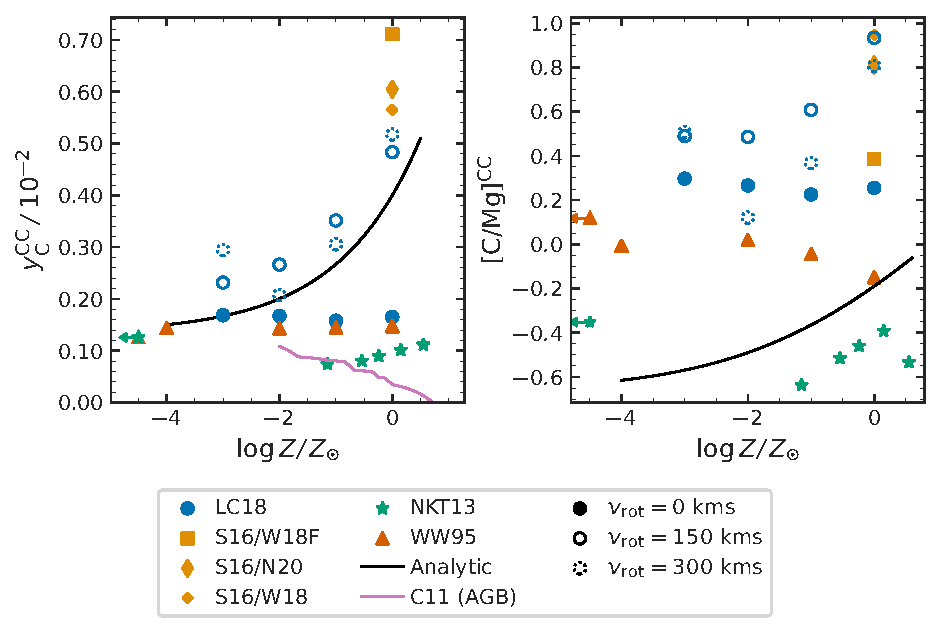
\includegraphics{cc_yields.pdf}
    \caption[]{
    \dbnote{y label: integrated CCSNe carbon yield}
        C yields from high-mass stars.
        \textbf{Left} The IMF-weighted \cc\ yield of C as a function of metallicity.
        \textbf{Right} The \cc\ [C/Mg] abundance ratio, defined in Eq.~\ref{eq:c_mg_cc}. The black line is the derived C yield from section \ref{sec:equilibrium} and Eq.~\ref{eq:y_cc}. Yields are shown for tables from 
    \citet[red triangles]{WW95}, \citet[orange square and diamond]{sukhbold+16}, 
    \citet[green stars]{NKT13}, and \citet[blue circles]{LC18}. \citet{sukhbold+16} report yields for different black hole landscapes, while \citet{LC18} provide yields at different rotational velocities.
    In the left panel, the pink line denotes $\Ycagb$ from \fruity{} for comparison. All models include wind yields. 
}
    \label{fig:y_cc}
\end{figure*}



\subsection{Equilibrium Abundances}\label{sec:equilibrium}

Building on \citepos{WAF17} analytic models of chemical equilibrium,
\citet{james+23} demonstrate that the relationship between N and O can be
explained by the metallicity dependence of their relative yields (see discussion
in their section 4.6).
We find similar results extending these arguments to C and Mg.
The equilibrium C/Mg abundance ratio is 
\begin{equation}\label{eq:equilibrium_yields}
    {\rm [C/Mg]_{eq}} = \log \left(\frac{\Ycc + \Ycagb }{y_{\rm Mg}}\right) - \log \left(\frac{Z_{\rm C,\,\odot}}{Z_{\rm Mg,\,\odot}}\right)
\end{equation}


We isolate the low-$\alpha$ sequence of subgiants to represent the equilibrium abundance trends, defined by [Mg/Fe] - [Fe/H] as in \citet{jack} (a +0.02 correction from \citet{weinberg+19}).
Low-$\alpha$ stars are defined as stars with
\begin{equation}\label{eq:high_alpha}
\begin{cases}
\text{[Mg/Fe]} <0.16-0.13\,\text{[Fe/H]}, & \text{[Fe/H]}<0\\
\text{[Mg/Fe]} <0.16, & \text{[Fe/H]}>0. \\
\end{cases}
\end{equation}
with high-$\alpha$ stars being otherwise from \citet{weinberg+19, weinberg+22, emily+19, emily+21}. \dbnote{I want to move this paragraph to \S 2.}

We propose the following functional form for total C yields near solar metallicities:
\begin{subequations}\label{eq:yc_inferred}
    \begin{align}
        \frac{\Yct(Z)}{y_{\rm Mg}} &\approx 4.20 + 1.64 \log (Z/\Zo)\\
        \frac{\Yct(Z)}{y_{\rm Mg}} &\approx 4.22 + 2.178 \log(Z/\Zo) + 5.53 \log(Z/\Zo)^2
    \end{align}
\end{subequations}
At solar metallicity, these yield ratios results in an equilibrium abundance $[{\rm C/Mg}] = -0.08$ which is consistent with our subgiant sample and is within \about{20\%} of the solar C/Mg mixture. 
For the quadratic form, we hold the yields constant past the vertex (at {\color{red} [M/H] = ?}) to avoid a premature upturn in \caah.
We discuss the choice of these functional forms more in appenix~\dbadd{X}.
In Fig.~\ref{fig:analytic}, we show the inferred C/Mg yield ratio against metallicity. 



\dbnote{check zetas}
With the total C yield of Eq.~\ref{eq:yc_inferred} and given an \agb\ C yield, we can derive an \cc\ C yield that would predict observationally consistant [C/Mg] ratios.
(by subtracting the assumed AGB contribution from the total yield fit above.)
\begin{subequations}
    \begin{align}
        \Ycc(\Zo) &= \Yct(\Zo) - \Ycagb(\Zo)\\
        \zeta &= \zcc + \zagb
    \end{align}
\end{subequations}
% \dbnote{I think I can get rid of the below equation.}
% \note{I'd suggest keeping it -- since you use $\zeta$ to distinguish between models, and it shows up in figure legends, the visibility of its exact definition will improve readability.}
where $\zeta$ is the (solar) metallicity dependence of the C yield at $Z=\Zo$
\begin{equation}
    \zeta = \frac{d y_{\rm C}}{d \log Z} \Big \vert_{(Z=\Zo)},
\end{equation}
and $\zcc$ and $\zagb$ correspond to the specific enrichment channels. 

Both observational and theoretical uncertainties limit the accuracy of our relative yield predictions. Additionally, the derived yields will be systematically biased if the galaxy is out of equilibrium, e.g. due to a recent starburst \citep{mor+19,isern19}. 


\section{The Multi-zone Model}\label{sec:vice}

Our models extends the \citet[hereafter \JJ]{james+21} Milky Way model, run with the publicly available Versatile Integrator for Chemical Evolution (\VICE).%
    \footnote{\VICE~is available at \url{https://github.com/giganano/VICE}}
This model is described extensively in \JJ~and concisely summarized  in \citet{james+23}. Here, we provide a brief overview of the relevant model components.

Classical, \textit{one-zone} models of chemical evolution assume instantaneous mixing of metals in the star-forming ISM\ \citep[e.g.][]{matteucci21}. This simple framework is a poor approximation of the Milky Way.  The Galaxy evolves \textit{inside-out} -- where star formation is higher towards the center and in the early universe \citep{WF91, kauffmann96, bird+13}. Stars can also migrate several kpc over their life/times, mixing different chemical environments across the galaxy \citep{bird+12,sellwood+binney02}. Multi-zone models account for stellar migration and changing environments by stitching together multiple one-zone models and mixing stellar populations. \dbnote{does this belong in intro or here?. Thinking here now because feels more like methodology justification, but not sure still.}

For our O, Mg, and Fe yields, we adopt the yields in \citet{david_fe}. We use a scaled variation of the AGB N yield from \citet{james+23} with a metallicity-independent CCSNe N yield. 
Following \citet{james+21, james+23}, we take the \ia{} delay time distribution to be a $t^{-1.1}$ power-law with a minimum delay time of 150\,Myr, as suggested by the observations of \citet{maoz+12}. 
\dbnote{discuss SNe Ia (maximum 4\% of C but likely much less) and SAGB (also minimal). Also: can novae produce any C?}


The Galaxy is divided into 200 rings, each representing a single, 100\,pc zone. Each ring (or zone) has a separate stellar population and gas supply. We initially assume an inside-out SFH from \JJ, where the star formation surface density $\dot{\Sigma}_\star$ is given by 
\begin{equation}\label{eq:inside_out}
    \dot{\Sigma}_\star \propto \left(1-e^{-t/\tau_{\rm rise}}\right) e^{-t/\tau_{\rm sfh}}.
\end{equation}
$\tau_\text{rise}=2$\,Gyr loosely describes when the star formation rate reaches a maximum, and $\tau_{\rm sfh}$ describes the decay timescale of star formation as a function of radius $R$. \JJ\ derive $\tau_{\rm sfh}(R)$ through analysis of four integral field spectroscopy surveys in \cite{sanches20}. At each $R$, the SFH is normalized to match the stellar surface density gradient \citep{BHG16} assuming a total stellar mass of $5.17\times10^{10}\,\Mo$ \citep{LM15}. Star formation ends beyond a radius $R=15.5\,$kpc, but stellar populations are allowed to migrate as far as $R=20\,$kpc.  
The gas inflow is calculated to maintain the SFH for each radius and time, using an extension of the Kennicutt-Schmidt law \citep{kennicutt98} motivated by the combined observations of \citet{bigiel+10} and \citet{leroy+13}, 
\begin{equation}
\dot{\Sigma}_{\star} \propto 
\begin{cases}
    {\Sigma}_{\rm gas} & 2\times 10^7 \Mo\,{\rm kpc}^{-2} \leq \Sigma_{\rm gas} \\ 
    {(\Sigma}_{\rm gas})^{3.6} & 5\times 10^6 \Mo\,{\rm kpc}^{-2}\leq \Sigma_{\rm gas} < 2\times10^7 \Mo\,{\rm kpc}^{-2}\\ 
    {(\Sigma}_{\rm gas})^{1.7} & \Sigma_{\rm gas} < 5\times10^6 \Mo\,{\rm kpc}^{-2}.
\end{cases}
\end{equation} 
The scaling of this relationship varies with time due to the redshift dependence of $\tau_\star$ in molecular gas observed by \citet{tacconi18}. We assume a \citet{kroupa01} IMF.


To account for radial migration, we use a normally-distributed, $\sqrt{\rm time}$ migration scheme. The final position of each star particle is sampled from
\begin{subequations}
\begin{align}
        R_{\rm end} &\sim N(R_{\rm birth}, \sigma_R ) \\
        \sigma_{R} &= 1.27\,{\rm kpc} \sqrt{\frac{t_{\rm end} - t_{\rm birth}}{1 \rm Gyr}}
\end{align}
\end{subequations}
At the boundaries, stars at $R=0$ move to $R=0$ if $R_{\rm end}<0$ and stars will move to $R=20$\,kpc if $R_{\rm end} > 20$\,kpc. 
The star moves from its birth radius to its final radius via
\begin{equation}
        R(t) = \Delta R \sqrt{\frac{t - t_{\rm birth}}{t_{\rm end} - t_{\rm birth}}}
\end{equation}
The $\Delta R \propto \sqrt{\rm time}$ dependence arises when migration proceeds as a consequence of the diffusion of angular momentum \citep{frankel18, frankel20}.
At each time step, each star particle travels a radial distance sampled from 
where $N(\mu, \sigma)$ represents a draw from normal distribution and $dt=20$\,Myr is the simulation timestep.%
\footnote{Not shown here, we also explored variations of temporal, spatial resolution, migration strength, and the mass lifetimre relation. We found these do not affect median trends significantly.}
We do not account for radial gas flows.
Not shown here, we also explore migration based on random walks and the \texttt{h277} hydrodynamical
simulation results\footnote{(with simulation parameters as in \citealt{bird+21}; see also \citealt{christensen12, zolotov12, loebman12, BZ14} \dbnote{is this okay as footnote?} }, which leaves our qualitative conclusions unchanged. 
The full impact of the details of a galaxy's dynamical history on its chemical evolution is still unknown.

As the strength of outflows controls the resulting $\alpha$-element abundances, we extend \JJ and create a metallicity gradient by defining
\begin{equation}\label{eq:mass_loading}
\eta(R) = \frac{y_{\alpha}^{\rm cc}}{Z_{\alpha}(R)} -1 + r + \tau_{\star} / \tau_{\rm sfh} 
\end{equation}
where 
\begin{equation}
    \log Z_{\alpha}(R) = \log Z_{\alpha,\ \odot} + 
    0.29 + 
    \begin{cases}
        -0.015(R-5) & R < 5 \\
        -0.09(R-5) & R \geq 5
    \end{cases}
\end{equation}
is adapted from \citet{hayden+14}.  We approximate $r=0.4$, and $\tau_\star/\tau_{\rm sfh} \approx 0.0$ \dbnote{double check this...}.
This choice of $\eta(R)$ results in a [$\alpha$/H] gradient consistent with Milky Way observations \citep[e.g.][]{hayden+14, weinberg+19, frinchaboy+13}.
If we change our assumed $y_{\rm Mg}$, the values of $\eta$ will change similarly to maintain the correct chemical trends.


Finally, we tune the carbon yields of CCSNe in slope and normalization to approximately match the median trends in most cases.
A tabulated description of our model parameters is available in appendix~\dbadd{model parameters}.

\section{Results}\label{sec:results}

\subsection{Evolution of Carbon Abundances}


\begin{figure*}
\centering
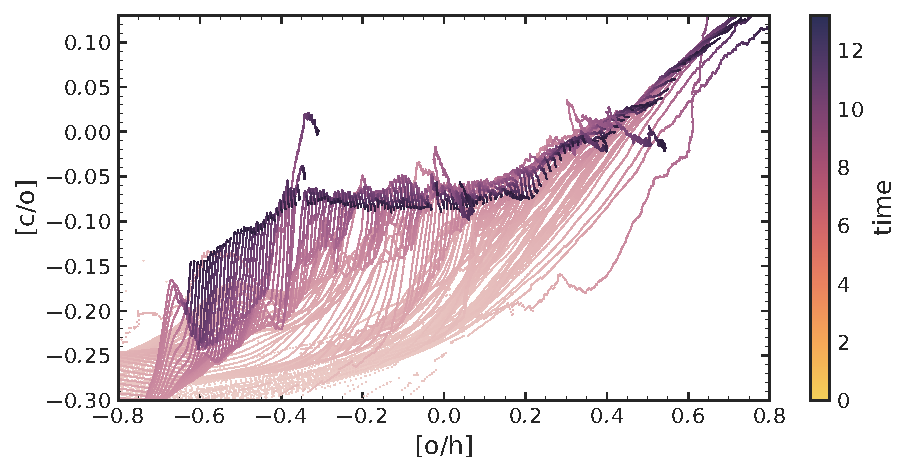
\includegraphics{figures/all_the_tracks.pdf}
\caption[]{
    Time evolution of gas-phase C abundances in our fiducial model for [C/Mg] versus [Mg/H] (left) and [Mg/Fe] (right).
    Each line represents a zone at a different galactic radius and is colour-coded by time. While \caah\ settles into the final trend $\sim{8}$\,Gyr ago, \caafe\ continues to evolve for much longer.
}
\label{fig:c_evo}
\end{figure*}



Fig.~\ref{fig:c_evo} shows evolutionary tracks for every zone of the fiducial model for [C/Mg] against [Mg/H] and [Mg/Fe].
\caah\ trend quickly reaches our equilibrium state in \about{5}\,Gyr. \caafe\ tracks continue to evolve due to the long tail in the DTD of \ia. 


The evolution of abundances in our fiducial model:
\begin{enumerate}
    \item[(1)] Star formation begins. Initially, \cc\ dominate enrichment. [C/Mg] evolves with yields set by $\Ycc/\Yoc$, resulting in increasing values with [Mg/H].  [Mg/H] quickly approaches its equilibrium value, but Fe remains low in comparison (in agreement with \citealt{WAF17}).
    \item[(2)]  A few hundred million years later,  delayed sources  enrich the ISM. \agb\ stars release C, raising [C/Mg], and \ia\ expel Fe, lowering Mg/Fe. 
    \item[(3)] Several billion years later, [C/Mg] plateaus as C also approaches equilibrium. [Mg/H] reaches equilibrium. [Fe/H] continues to incrase due to ongoing \ia\ from old stellar populations.
    \item[(4)] In the final few billion years, [C/Mg] decreases slightly due to declining \agb\ C yields. \caah\ trends shift only slightly, and [Mg/Fe] slowly and steadily decreases.

\end{enumerate}


This evolution is driven most dominantly by our chosen elemental yields, their
dependence on metallicity, and their DTDs.
As we will demonstrate in section 5.2 below, the slope of the [C/Mg]-[Mg/H] trend is
set by the relative contributions of CCSNe and AGB stars to the overall C abundance.
The positive metallicity dependence of massive star C yields outweighs the negative
dependence of AGB star yields, causing [C/Mg] to increase with [Mg/H].


To create representative stellar samples to compare with APOGEE, 
We draw \nsubgiants\ stars from the simulated stellar populations such that the selection probability is proportional to a stellar population's mass and that the subsample follows the same distribution in Galactocentric radius as the subgiants. 
Fig.~\ref{fig:equilibrium_validity} displays our sample of stars and compares them to analytic representations of the mean trend. 
The median sequence of the low-$\alpha$ stars closely follows the {\it equilibrium track}, defined by the ratio between total C and Mg yields at each metallicity. There is a slight ($\sim{0.02}$ dex) divergence between the median track and equilibrium at higher metallicities, caused by our particular choice of C yields and the finite time it takes to reach equilibrium especially at higher metallicities with an increasing yield. However, if the low-$\alpha$ sequence is approximantly matched by our {it total} C yield, then we expect our model to agree with stellar observations.
On the other hand, in \caafe\ equilibrium is a vertical line. As we assume both Mg and Fe yields are metallicity independent, there is only one value of [Mg/Fe] in the equilibrium sequence, corresponding to the low-$\alpha$ population. The median trend here instead reveals the delay time distribution of C, revealed by the green single-zone model included. 

Galactocentric radii are taken from astroNN {\color{red} citation}. \dbadd{Using Gaia parallaxes does not affect our conclusions ?}



% note about \caafe plane
% As low-$\alpha$ stars were formed in regions closer to chemical equilibrium, we only plot the medians of the low-$\alpha$ sequences in \caah. 
% Instead, \caafe\ trends are set by the proportion of \agb\ C contribution. The \caafe{}-diagram, when restricted to a narrow range of metallicities, becomes an empirical delay-time-distribution of C. 
% High-$\alpha$ stars were formed in regions further from chemical equilibrium than stars with low [Mg/Fe]. Immediately after a star formation event, \cc\ elements dominate and only after sufficient time do \ia\ elements like Fe reach their higher-equilibrium abundances. 
% Likewise, high-[Mg/Fe] stars will have a greater portion of \cc\ C, as low-[Mg/Fe] stars will include more \agb\ C. 
% When binned in metallicity, median [C/Mg] changes by about 0.2 dex across the range of [Mg/Fe] at solar metallicities. As high-$\alpha$ stars have little to no delayed \ia\ Fe, these stars would also have little to no delayed \agb\ C. This means that AGB C stars make up about at most a fraction $f_{\rm agb} \approx 1 - 10^{-0.2} \approx 0.4$ of C production.
% 
% \begin{figure}
%     \centering
%     \includegraphics{apogee_caafe_binned.pdf}
%     \caption{Caption}
%     \label{fig:caafe_binned}
% \end{figure}

\subsection{Yield Variations}\label{sec:results_highmass}
\label{sec:agb_results}


\begin{figure*}
    \centering
    \includegraphics{figures/subgiants_equilibrium_reproduced.pdf}
    \caption{Similar to Fig.~\ref{fig:subgiants} except for the stars of our fiducial model. 
    The solid, black lines show the equilibrium abundance track. The black scatter points with errorbars are the median bins for the low-$\alpha$ sequence (left) and the \caafe\ trend (right). The green solid line on the right shows the singlezone evolution of \caafe\ with properties matching our solar-annulus. The median trend of low-$\alpha$ stars is an excellent approximation for the equilibrium abundance of C. 
    \dbnote{we add synthetic scatter found by fitting the metallicity-dependent reported errors with a linear fit in APOGEE and adding gaussian noise.}
    \dbnote{is there too much going on here?}
    \label{fig:equilibrium_validity}
    }
\end{figure*}




\begin{figure*}
\includegraphics{sims_zeta_f.pdf}

\caption[]{
    Stellar abundance trend predictions of our models . Coloured lines represent the median [C/Mg] in bins of [Mg/H] (left) or [Mg/Fe] (right) for each \agb\ table. Black points and grey dashes represent the median and 16th-84th percentiles of [C/Mg] in each bin in the \citet{jack}~sample. 
    The left panel only shows low-$\alpha$ stars. In the right panels, we show the trends only for stars where $-0.15\leq {\rm [Mg/H]}\leq -0.05$.
    Stars are binned into 20 (left) or 12 (right) equal number bins. 
    \textbf{Top}: Models with different metallicity dependences for  \cc\ C yields. \textbf{Bottom}: Different \agb\ fractinos of C.
}
\label{fig:zeta_f}
\end{figure*}


\begin{figure*}
\includegraphics{figures/zeta_f_mass_sfh.pdf}

\caption[]{
    Similar to Fig.~\ref{fig:zeta_f}, except for \caafe\ for a variety of models.
    {\bf Left} models where both the \agb\ fraction and the CCSNe slope are varied simultaneously.
    {\bf Middle} models where the \agb\ yields are shifted by some factor in mass.
    {\bf Right} alternate star formations and a model where yields and outflows are $\sim$ doubled.

    \dbnote{I looked into the halfed yields model. Since in this paper, we assume $y_o/Z_o \sim 1$, it is essentially impossible to reach solar Z when halfing the yields. I am swapping for all yields are doubled and I think if a referee complains about our choice of $\eta\sim0.4 \ne 0$ at the sun, we can deal with that later}

    \dbnote{middle pannel is reproduced in analytic multizone models. low-priority but possibly interesting is if the analytic DTD or singlezone models reflect this trend as well.}
}
\label{fig:sims_degens}
\end{figure*}




The top of Fig.~\ref{fig:zeta_f} shows models with varying strengths of the $\Ycc$ metallicity dependence, $\zcc$. With higher $\zcc$, the model predicts a steeper \caah\ trend, owing to the direct relationship between the C/Mg equilibrium abundances and yield ratios. 
However, \caafe~is minimally affected by changes to $\zcc$ since \cc\ occurs on much shorter timescales than \ia\ and \agb\ enrichment.%
\footnote{The only effects on \caafe, when considering the narrow metallicity slice, are because of either the systematic change in equilibrium abundances, the imperfect evolution of the galaxy, or that the ISM abundances are set by stars which were born at poorer metallicities. }
%  Hence, \caah\ tells us about the total C yield with metallicity, which \caafe\ is independent of. If we know the \agb\ C yields, then with observed \caafe\ abundance trends, we can infer the \cc\ C yields with metallicity.



The bottom of Fig.~\ref{fig:zeta_f} shows three models with different C \agb\  fractions, defined as 
\begin{equation}\label{eq:f_agb}
    \fagb \equiv \frac{\Ycagb(\Zo)}{\Yct(\Zo)}.
\end{equation}
Modifications of $\fagb$ affect both \caafe\ and \caah. At fixed metallicity, the \caafe\ trend is principally sensitive to how much C and Fe comes from delayed sources. Increasing the \agb\ fraction therefore steepens the \caafe\ trend as expected. Though each yield model predicts the trend to flatten at ${\rm [Mg/Fe]} \lesssim 0.1 $, the median is still within the width of the observed distribution and the overall agreement is good. Additionally, increasing \agb\ contribution to C leads to a declining net slope for the total C yield owing to the negative slope of \agb\ C production with metallicity.

Because both the increase in \cc\ slope $\zcc$ and AGB fraction $\fagb$ have similar impacts to \caah, we can change both parameters simultaneously to retain agreement in \caah. We show example models in the left panel of Fig.~\ref{fig:sims_degens} in \caafe, (as models cannot be readily distinguished in \caah). The principle effect of increasing $\fagb$ and adjusting $\zcc$ correspondingly is to increase the amplitude of the trend in \caafe. Models with little to no AGB C production will produce stars with [C/Mg] independent of [Mg/Fe] in a metallicity slice. As the AGB fraction increases to an extreme $f^{\rm AGB}=0.5$, the trend becomes much steeper than the fiducial but remains a mere rescaling of the same shape. 


A second factor affecting \caafe\ is the assumed delay time distribution of \agb\ carbon production.
The middle panel of Fig.~\ref{fig:sims_degens} shows models where the AGB yields have been shifted by some factor in mass. When the AGB C production is weighted towards more massive AGB stars, then the delay time distribution becomes more like CCSN. As such, the predicted \caafe\ trend resembles the model which only contains CCSN production. The \caafe\ trend therefore is much less sensitive to the C production by stars with masses $M \gtrsim 5 \Mo$. On the other hand, shifting the C production towards low mass stars changes both the shape and amplitude of the DTD. This is evident in a transition point, where the \caafe\ trend changes slope. For the most extreme case, where the masses are shifted by a factor of 0.5; the AGB production is more delayed than SNeIa, causing a steepining of \caafe\ towards low [Mg/Fe]. Intermediate values are more linear in \caafe, matching the observed trend. We note that the fiducial model instead transitions from steep to shallow as [Mg/Fe] decreases. This is evidence that AGB C likely needs to be weighted more towards low mass stars than is predicted by current AGB stellar models.

Considering the effects of changes in the amplitude and mass of AGB C production, we can now predict and understand the differences between different yield tables.
Fig.~\ref{fig:agb_predictions} show the four C yield models (\fruity, \aton, \monash, \nugrid, with no scaling). For the most part, different \agb\ yield tables result in qualitatively similar predictions. While small adjustments in the \cc\ yields results in identical tracks through \caah, each model predicts slightly different tracks in \caafe. Differences are due to the total C production from the AGB model, and the delay time distribution of the model. For example, V13 predicts that AGB stars produce almost net zero C at solar metallicity, and \monash\ predicts the shortest delay time distribution of all models. These models thus are almost consistent with pure \cc\ enrichment of C. Additionally, \nugrid\ yields are about double \fruity, resulting in a steeper slope in \caafe.
%\aton, however, does not reproduce solar trends as the model predicts strong C destruction at slightly super-solar metallicities, resulting in inversions in both \caah\ and \caafe. 
As all \agb\ models predict C yields to decline with metallicity, all models predict an increasingly downward slope in \caafe\ with [Mg/Fe]. A recent burst in star formation may hide this downturn (see section~\ref{sec:sfh}), but C destruction at the level predicted by \aton\ is not supported by our sample. 
Because the effects of alternate \agb\ yield sets are small, we focus on \fruity{} model for the remained of this paper. Alternate yield sets minimally affect our conclusions. 


\dbadd{the inter-study differences for AGB yields can be explained by the differing mass dependence, and the metallicity dependence.}


\subsection{Variations in Star Formation History} \label{sec:sfh}
In this section, we consider an alternate SFH, namely one which exhibits a late-time elevation in the star formation rate. Motivated by the findings of \citet[see discussion in \JJ]{mor+19,isern19}, this \textit{lateburst} model
adds a Gaussian burst to the fiducial inside-out model, 
\begin{equation}\label{eq:lateburst}
    \dot{\Sigma}_\text{lateburst} \propto \dot{\Sigma}_\text{inside-out} \left(1 + A\,e^{-(t-\tau_{\rm burst})^2/2\sigma^2_{\rm burst}} \right)
\end{equation}
where $A=1.5$ represents the amplitude of the birth, $\tau_\text{burst}=10.8$\,Gyr is the time where the burst is strongest, and $\sigma_\text{burst}=1$\,Gyr is the width of the burst.

We additionally consider a two-infall like model as presented in \dbadd{dubay + 24}, which is defined as.

\begin{equation}\label{twoinfall}
\dot{\Sigma}_{\rm in} \propto exp(-t/\tau_1) + A_{2,1} \theta(t - t_{1}) \exp(-t/\tau_2)
\end{equation}

where $\tau_1=0.4\,$Gyr, $\tau_2$ is 1/2 of the value from Sanchez, $A_{2,1}=0.5$, $t_1=4.1$, and the star formation also abruptly transitions from $\nu=2$ to $\nu=1$ at $t=t_1$.

The right panel of Fig.~\ref{fig:sims_degens} compares the fiducial, lateburst, and two-infall models. The lateburst slightly shifts \caah\ down and only slightly perturbs \caafe. These variations are small compared to the width of the observed distribution. 
Building on \citet{james+23}, we therefore conclude that the \caah\ and \caafe\ trends reflect nucleosynthetic yields more than the Galactic SFH. 

\dbnote{there has to be a good reason why \caafe\ is not affected or maybe only more extreme pertubations make a difference?}



\subsection{Degeneracies} \label{sec:outflows}

While some Milky Way \gce{} models (including ours) incorporate significant mass-loading, others
neglect mass-loading and instead use lower yields \citep[e.g.][]{MCM13, MCM14, spitoni19, spitoni20, spitoni21}.
Both classes of models are able to reproduce many details of the disk abundance structure due to the strong degeneracy between the normalizations of elemental yields and mass-loading (see discussion in, e.g. \citealt{sandford+24} and appendix B of \citealt{james+23}). 
Our parameterization of $\eta$ illustrates this (see Equation~\ref{eq:mass_loading}) -- choosing a lower value of $y_{\alpha}$ will similarly result in lower values of $\eta$ while maintaining the same metallicity gradient. 
We consider a model where we double all yields, in the right panel of Fig.~\ref{fig:sims_degens}. A uniform change in yields and outflows leaves our median trends relatively unchanged. 

\dbnote{paragraph about how fagb and zeta are interdependent, but not fully degenerate in \caafe.}

Additionally, Fe yields and the \ia\  delay-time-distribution have their own uncertainties. Increasing both $y_{\rm Fe}^{\rm Ia}$ and $\Ycagb$ correspondingly leaves \caafe\ mostly unchanged. Not shown here, if both processes increase by a similar proportion of the total yield, then our predictions in \caafe\ are unchanged. Therefore, we cannot know the DTD of C much better than that of Fe in this framework.


\dbnote{Other things to discuss possibly ? :
 Initial mass function (and possible metallicity dependence)? Metallicity dependent Oxygen/Magnesium and Iron yields? Gas phase migration / ISM cooling?  MLR
 }


\subsection{Nitrogen}


\begin{figure}
\centering
\includegraphics{figures/nitrogen.pdf}

\caption[]{Similar to Fig.~\ref{fig:zeta_f} except for [C/N] against [Mg/H] for the fiducial model. Combining our results with the suggested yield from \JJ\ (rescaled to our adopted yields) explains both the thin-disk evolution of C and N. 
}
\label{fig:nitrogen}
\end{figure}

N production, also affected by the CNO cycle, is closely tied to C. As a test of our model, we use the \agb\ N yield suggested by \citet{james+23}. Fig.~\ref{fig:nitrogen} shows [C/N] versus [Mg/H] and for our fiducial model. We are able to closely match the [C/N]-[Mg/H] trend. 




\section{Gas-Phase Abundances}\label{sec:gas}

\begin{figure*}
\centering
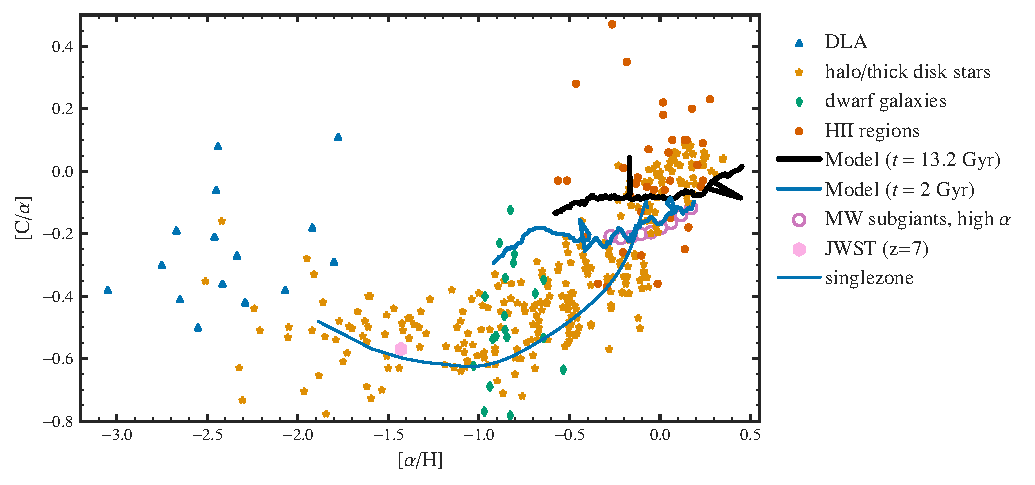
\includegraphics[]{figures/summary.pdf}
\caption[]{\dbnote{warning: caption in progress} 
Gas-phase C abundances. 
We plot the fiducial model's present-day ISM abundances as a thick blue line (\protect\captionline[line width=1.5pt]{blue}).
Black lines are single-zone models: a fiducial yields and MW-like model (solid black), and three corrected yield models representing the MW (dotted), GSE (dashed) and Wukong (dash-dots).
Points represent measurements in 
    HII regions \citep[orange circles;][]{skillman+20, esteban+02, esteban+09, esteban+14, esteban+19}
    damped Lyman-alpha (DLA) systems \citep[rust triangles;][]{ellison+10, srianand+10, dutta+14, DZ+03, pettini+08, morrison+16,cooke+17}, ({\color{red} citations})
    dwarf galaxies \citep[green diamonds;][]{berg+19},
    Milky Way stars \citep[yellow stars;][]{amarsi+19},
    and high redshift galaxies \citep[pink squares;][]{arellano-cordova+2022} ({\color{red} citations}).


}

\label{fig:gas_phase}
\end{figure*}
% \begin{table}
% 	\centering
%     \caption[]{Single zone model parameters. \dbnote{change dwarf parameters to match Wukong from James' dwarf paper.  $\eta=47.99\pm 5$, $t_{\rm end} = 3.36\pm 0.5$, $\tau_\star=44.97\pm 7$, $\tau_{\rm sfh} = 3.08\pm 1$}}
% 	\label{tab:singlezone_params}
% 
% 	\begin{tabular}{l l l l l}
% 		\hline
%         Model & $\eta$ & $t_{\rm end}$ & $\tau_\star$ & $\tau_{\rm sfh}$ \\
% 		\hline
%         1 & 0.5 & 13.2 & 2.5 & 14\\
%         2 & 1 & 10 & 2 & 10\\
%         3 & 9 & 3 & 5 & 3\\
% 	\end{tabular}
% \end{table}

As a final test of our model, we compare the predictions against C abundances
in the gas-phase.
These measurements are challenging since C lacks strong collisional excitation
lines, and its recombination lines fall in the ultraviolet with no nearby
H lines to reference~\citep[e.g.,][]{skillman+20}.
These two classes of spectral lines are also systematically discrepant at the
factor of~$\sim$2 level~\citep{GR07}.
As a consequence, the uncertainties associated with any one measurement are
substantial (see the representative error bars in Fig. 13), but we are able to
illuminate the underlying mean trends by combining observations from multiple
sources.
\dbnote{I believe that dust might warrent a discussion here since this can capture gas-phase metallicity, substantially affecting observations. But we also just don't know how to measure gas-phase abundances well at all. Reassuring as it means that our focus on stars is very justified.
There is an additional complication that CEL and RL abundances (especially for O) need to be put on the same scale with +0.2 dex corrections, and there is not a clear understanding which one is better.
\citet{MM19}
}

\dbnote{does it make sense to include more high-redshift galaxies? 
Many of these seem to be through stacked spectra or other challenging measurments, e.g. redshifting the CEL lines in Berg++ dwarfs at $z\sim 2$
}

DLAs are .......
Most similar tothose in local group dwarfs (Cooke+2015, berg+2015, cia+2016 from MM2019 review).


Fig.~\ref{fig:gas_phase} shows our compilation alongside the gas-phase abundances in our model
at snapshots of~$t = 2$ Gyr and the present day.
While we used Mg as our representative alpha element in our APOGEE sample, O
is more readily observed in the gas-phase, so we shift focus to C/O in this
section.
The model at the present day is consistent with the mean trend seen in HII
regions in the MW and similar star forming galaxies at redshift~$z \sim 0$.
Together with our results in~\S~5, this agreement suggests that our yield model
is an accurate description of C nucleosynthesis at metallicities typical of
MW-like galaxies.

Nonetheless, our model does not extend as low in metallicity as dwarf galaxies
or (especially) damped Lyman-alpha systems.
To test our model at these abundances, we show 4 different one-zone GCE models.
\begin{enumerate}
    \item Fiducial MW: $\eta=0.5$, $t_{\rm end} = 13.2$, $\tau_\star=2$, $\tau_{\rm sfh} = 14$
    \item Corrected MW-like. 
    \item Corrected Gaia-Sausage Enceledus like. $\eta=9.56$, $t_{\rm end}=10.73$, $\tau_\star = 26.60$, $\tau_{\rm sfh} = 2.18$, infall mode
    \item Corrected Wukong-like: $\eta=47.99\pm 5$, $t_{\rm end} = 3.36\pm 0.5$, $\tau_\star=44.97\pm 7$, $\tau_{\rm sfh} = 3.08\pm 1$, infall modej
\end{enumerate}
with the exception of the fiducial like model, we use the bi-log-linear CCSNe yield model which plateaus at a [C/Mg] at low metallicity consistant with observations of metal-poor stars and dwarf galaxies.
\dbnote{check timescales to metallicity = -1 (could sagb affect the trends here?). Also try different yield sets for these just to see if any agree naturally... }

Fig.~\ref{fig:gas_phase} also plots a single-zone model and time-slices of the fiducial multi-zone models gas-phase at present day and $t=2$\,Gyr. 
Our single-zone model is designed to have parameters broadly consistent with the Gaia-Encelidus sausage.
We evolve the singlezone model for 2\,Gyr, using mass loading $\eta=20$, star formation efficiency $\tau_{\star}=30\,{\rm Gyr}$, and a star formation history $\propto e^{-t/3{\rm\,Gyr}}$.
The single-zone model uses a 1.5 mass factor times f=0.25 C11 yields. Note that the mass shift results in significant C destruction by high-mass AGB stars at low metallicities, enabling the model to reproduce the low [C/O] abundances at [O/H] = -1.


Each of these one-zone models predicts a steeper C/O-O/H trend than our
fiducial multi-ring model from previous sections.
This difference arises because the trend in the multi-ring models arises as a
superposition of end-points (see Fig.~\ref{fig:c_evo}), qualitatively similar to, e.g.,
\citepos{schonrich-binney09} argument regarding
the low-alpha sequence.
In the one-zone models, the trend instead arises as an evolutionary sequence.
To demonstrate this point further empirically, Fig.~\ref{fig:gas_phase} includes measurements
in halo and thick disk stars.
This sample indeed shows a C/O-O/H trend that is clearly steeper than our
fiducial multi-ring model, which is an accurate representation of the APOGEE
low-alpha sequence (see Fig. 8).

At the lowest metallicities ($\log_{10}(Z / Z_\odot) \lesssim -2$), our suite
of one-zone models is consistent with the C/O ratios seen in damped Lyman-alpha
systems.
For all parameter choices, these ratios simply reflect the relative C and O
yields of low-metallicity massive stars (see Fig. 5), with the increase in C/O
at higher metallicities arising due to the onset of AGB star enrichment (see
Fig. 7).
As a consequence, our yield model as parameterized predicts that C/O ratios
should never be significantly below~$\sim$half solar.
This prediction is challenged by the measurements in both dwarf galaxies and
halo/thick disk stars in Fig.~\ref{fig:gas_phase}, which suggest ratios~$\sim$$0.2 - 0.3$ dex
below solar between~$\log$(O/H) = X and Y.

This discrepancy could arise at least in part due to failures of our yield
prescription and, by extension, could point to shortcomings in stellar
nucleosynthesis models.
However, we cannot rule out the possibility of systematic uncertainties in
abundance determinations playing a role.
At these metallicities, deviations from local thermal equilibrium (LTE) can
bias measurements at the~$\sim$0.2 dex level~\citep[e.g.,][]{amarsi+19}.
Considerations of non-LTE effects are not included in our APOGEE sample, but
the corrections are smaller near solar metallicity.

\dbnote{Discussion on a complex landscape of C production: elevation at lowest metallicities but with stochastic mixing, Pop III and many other problems; declining at [O/H] = -1, increasing due to Z-dependent CCSNe and delayed AGB enrichment up to 0, and flat in disks due to chemical equilibrium, but maybe also more flat CCSNe too.}


\dbnote{depending on what everyone thinks, may be worth discussing CEMPs since they have enough literature although not necessarily relavent here. Carigi+Peimbert 2011, Molla+2015. Lyman limit systems in Lehner+2016.}


\dbnote{other stellar surveys...
Gustafsson+1999, bensby\&feltzing+2006, Spite+2005, Neiva \& Przybilla+2012, Tautvaisiene+2016.}



\section{Conclusions}\label{sec:conclusions}


Building on~\citet{james+23}, we quantify the impact of C yield assumptions on Milky Way GCE models. We use \citepos{jack} sample of APOGEE subgiants as our primary observational benchmark, as subgiant atmospheres most likely reflect their birth C abundances (see discussion in section~\ref{sec:data_selection}).
In our fiducial model, C initially increases following the slope of the \cc\ C dependence. Later, AGB contributions from C cause a sharp rise in \caah, which slows down due to declining AGB C production and the approach towards equilibrium. The chemical elemental reach a quasi-equilibrium within \about{5}\,Gyr. As a result, the current C/Mg versus metallicity gradient is a superposition of equilibrium states, mixed together from different Galactic positions.


The slope of the predicted \caah\ relation is principally sensitive to the collective metallicity dependence of \cc\ C yields.
While AGB yields are predicted to decline with metallicity, out models show that \cc\ dominate the trend and make an overall positive metallicity trend. 
As the strength of the \cc\ metallicity dependence increases, the slope of the \caah\ trend correspondingly increases. The small effects of \agb\ C yield on the \caah\ trend can be easily corrected by small adjustments of the \cc\ yield's metallicity dependence.
Our predicted slope of NUMBER is approximately consistent with the \citet{LC18} rotating stellar models, however no simulation contains sufficient mass resolution or accuracy to reproduce the observed trends accurately. 

Because massive star enrichment dominates the C mass budget in our models, the predictions are relatively insensitive to the choice of AGB star yield model.
Of the \agb\ tables tested here, \fruity, \monash, and \nugrid\ all predict similar abundance trends in [C/Mg] with [Mg/H] and [Fe/Mg]. The strong destruction of C by massive stars at \about{} solar metallicity   in \aton\ are instead in tension with the data (See Figs.~\ref{fig:agb_predictions})  and~\ref{fig:agb-ssp})
As both the \fruity\ and \nugrid\ models predict \about{} linear N yields as well, these combined models best explain combined C and N abundance trends (see Appendix!?).

As in~\citet{james+23}, we have constrained yield ratios as opposed to absolute yields. For example, scaling yields and outflows by a corresponding factor leaves abundance ratio trends unchanged (Fig.~\ref{fig:sims_degens}).  Effects such as black hole formation could create systematic shifts on predicted chemical yields.
Variations in the SFH instead only induce minor systematic shifts


When combined with~\citeauthor{james+23}'s~\citeyearpar{james+23} empirically calibrated N yields, we find that our fiducial model accurately describes the [C/N]-[Mg/H] relation in our sample. The [C/N]-[Mg/Fe] relation, on the other hand, is shallower than the data, indicating that the DTD of C production may be sharper than our AGB yield tables would suggest (or the N DTD more extended, or both).

Finally, we compare our models againsts a compilation of literature gas-phase and halo-star abundances (see Fig.~\ref{fig:gas_phase}). Our fiducial model fails to explain the lowest values of [C/O] at metallicities of -1 to -2. We briefly consider a modified variation of the CCSNe yield of C which drops to explain these values, which maintains trends consistant with APOGEE. 


Our results demonstrate the power of empirically calibrated stellar yields. In our GCE models, trends in abundance ratios with metallicity are largely determined by trends in yield ratios with metallicity. As a result, the metallicity dependence of the total, population-averaged C yield is tightly constrained by the [C/Mg]-[Mg/H] relation, but the metallicity dependencies of the individual contributions from CCSNe and AGB stars are less precisely determined. Due to the sensitivity of elemental yields to poorly understood processes, such as mass-loss rates and convection, our results provide a useful benchmark for stellar evolution models~\citep[see the discussion in e.g.][]{gil-pons+2022}. With abundance measurements for several million stars provided by upcoming spectroscopic surveys, particularly SDSS-V's Milky Way Mapper program~\citep{sdssv}, constraints on both stellar nucleosynthesis and the assembly history of our Galaxy will become increasingly more powerful.

More C observations across different galactic environments will continue to refine a complete understanding of C production, including the yields of the first stars,  evolution in the bulge, and so on. 



\section*{Acknowledgements}

Software that has contributed to this work included  
\VICE~\citep{JW20, james+21},
\textsc{matplotlib} \citep{matplotlib},
\textsc{scipy} \citep{scipy},
\textsc{IPython} \citep{ipy},
\textsc{pandas} \citep{pandas},
\textsc{numpy} \citep{numpy},
\textsc{astropy} \citep{astropy:2013, astropy:2018, astropy:2022},
and 
\textsc{seaborn} \citep{seaborn}
.
Additionally, we thank \citet{OhioSupercomputerCenter1987} for the use of its facilities for the simulations. 

\apogee\ is part of SDSS-IV \citep{sloan_telescope, apogee_instrumentation, sdss_iv_overview, sdss17, apogee17, aspcap}.

Funding for the Sloan Digital Sky 
Survey IV has been provided by the 
Alfred P. Sloan Foundation, the U.S. 
Department of Energy Office of 
Science, and the Participating 
Institutions. 

SDSS-IV acknowledges support and 
resources from the Center for High 
Performance Computing  at the 
University of Utah. The SDSS 
website is www.sdss4.org.

SDSS-IV is managed by the 
Astrophysical Research Consortium 
for the Participating Institutions 
of the SDSS Collaboration including 
the Brazilian Participation Group, 
the Carnegie Institution for Science, 
Carnegie Mellon University, Center for 
Astrophysics | Harvard \& 
Smithsonian, the Chilean Participation 
Group, the French Participation Group, 
Instituto de Astrof\'isica de 
Canarias, The Johns Hopkins 
University, Kavli Institute for the 
Physics and Mathematics of the 
Universe (IPMU) / University of 
Tokyo, the Korean Participation Group, 
Lawrence Berkeley National Laboratory, 
Leibniz Institut f\"ur Astrophysik 
Potsdam (AIP),  Max-Planck-Institut 
f\"ur Astronomie (MPIA Heidelberg), 
Max-Planck-Institut f\"ur 
Astrophysik (MPA Garching), 
Max-Planck-Institut f\"ur 
Extraterrestrische Physik (MPE), 
National Astronomical Observatories of 
China, New Mexico State University, 
New York University, University of 
Notre Dame, Observat\'ario 
Nacional / MCTI, The Ohio State 
University, Pennsylvania State 
University, Shanghai 
Astronomical Observatory, United 
Kingdom Participation Group, 
Universidad Nacional Aut\'onoma 
de M\'exico, University of Arizona, 
University of Colorado Boulder, 
University of Oxford, University of 
Portsmouth, University of Utah, 
University of Virginia, University 
of Washington, University of 
Wisconsin, Vanderbilt University, 
and Yale University.

\dbnote{do I need acknowledgements for appendix spectro-surveys?}

%%%%%%%%%%%%%%%%%%%%%%%%%%%%%%%%%%%%%%%%%%%%%%%%%%
\section*{Data Availability}

\dbadd{data and codes used in this paper are all publicly available. (do i need links here?). }


%%%%%%%%%%%%%%%%%%%% REFERENCES %%%%%%%%%%%%%%%%%%
\bibliographystyle{mnras}
\bibliography{main}


%%%%%%%%%%%%%%%%% APPENDICES %%%%%%%%%%%%%%%%%%%%%

\appendix

\section{Model Parameters}

\begin{table*}
	\centering
    \caption[]{Description of the models presented in this paper.}
	\label{tab:model_parameters}

	\begin{tabular}{l l l l l}
		\hline
            name & $Y_{\rm C}^{\rm AGB}$ & $y_{\rm C}^{\rm CC}$ & additional parameters \& notes \\
            \hline
            fiducial & 1.45 x fruity & $0.002203 + 0.00196x + Ax^2$ & default model. See Section~X.X \\
            FRUITY & 1 x fruity & $0.0024 + 0.002x + Ax^2$ \\
            Monash & 1 x monash & $0.0024 + 0.0025x + Ax^2$ \\
            ATON & 1 x aton & $0.00255 + 0.0025x + 0.0021 x^2$& \\
            NuGRID & 1 x nugrid(M, Z) & $0.0024 + 0.00136x + 0.0016x^2$& \\
            f=0.0 &  \\
            f=0.5 & 3.623 x fruity & $0.00138 + \zeta x + Ax^2$ & \\
            steep & 1.45xfruity & $zeta=$ \\
            shallow & 1.45xfruity & $zeta=0$ \\
            fz=0 \\
            fz=0.5 \\
            m0.5 & 1.44 fruity(m/0.5, Z)  & 0.00225 " & \\
            m0.8 & 1.44 fruity(m/0.8, Z) & " \\
            m1.5 & 1.44 fruity(m/1.5, Z) & 0.002194 " \\
            m2 & 1.44 fruity(m/2, Z) & 0.2587 " \\
            lateburst & & & SFH$\sim {\rm insideout} (1+N(t, 13.2, 1))$\\
            twoinfall & & & SFH$\sim$ ... , ... \\
            2y & & & all yields doubled;  $\eta$ adjusted to Eq.~N \\
            lowz correction& other equation & --- & --- \\
		\hline
	\end{tabular}
\end{table*}



For our added scatter, we use the polynomial fits to the reported internal APOGEE error with metallicity. In detail, these polynomials should also very with logg, teff, however as all of our stars are subgiants, these effects should be smaller. We also use $x={\rm [Fe/H]}$ for brevety.
\begin{subequations}
\begin{align}
    \delta {\rm [Mg/H]} &= 0.0652 x^2 + 0.00522 x + 0.0338 \\
    \delta {\rm [Mg/Fe]} &= 0.00793 x^2 - 0.00802 x + 0.0138 \\
    \delta {\rm [C/Mg]} &= -0.0378x + 0.03506 
\end{align}
\end{subequations}



\begin{figure*}
\includegraphics{sims_agb.pdf}

\caption[]{
    Similar to Fig.~\ref{fig:zeta_f}. 
}
\label{fig:agb_predictions}
\end{figure*}

The best fits assuming perfect equilibrium.
\begin{subequations}
    \begin{align}
        \frac{\Yct(Z)}{y_{\rm Mg}} &\approx 4.20 + 1.64 \log (Z/\Zo)\\
        \frac{\Yct(Z)}{y_{\rm Mg}} &\approx 4.12 + 1.21 \log(Z/\Zo) + 3.07 \log(Z/\Zo)^2
    \end{align}
\end{subequations}

\begin{figure}
    \centering
    \includegraphics{figures/equilibrium_yields.pdf}
    \caption[]{Inferred total C yields as a function of metallicity. We assume chemical equilibrium (orange curve, see discussion in section \ref{sec:equilibrium}). Blue points are the median value of $\Ycc$ for each (number) bin in [Mg/H] with uncertainties based on the 16--84 percentile range.
    \note{I'd rephrase this caption slightly to be a little more specific about what the lines are representing. Something to the effect of "The orange solid and green dashed curves show fits to the blue points under the assumption of a chemical equilibrium trend (see discussion in section \ref{sec:equilibrium}).
    }

    \dbnote{Considering cutting this figure (requires about 0.1 dex adjustment and compare to Fig.~\ref{fig:equilibrium_validity})}
    }
    \label{fig:analytic}
\end{figure}




\bsp	% typesetting comment
\label{lastpage}
\end{document}




